\section{Modellierung physikalisches System}\label{kap:physikalisches_system}
Ein Stoss kann für die Simulation mithilfe eines Modells beschrieben werden.
Dieses Modell beschreibt den Ablauf eines Stosses durch Ereignisse, welche den beteiligten Objekten wiederfahren.
Die Kugeln, Banden und Löcher sind die Objekte dieses Modells.
Jedes Objekt dieses Modells hat einen veränderlichen Energiewert, bsp. sind Kugeln in Bewegung oder sie sind ruhend.
Eine Bande oder ein Loch bewegen sich nie, d.h. deren Energiewert ist konstant 0.
Kollisionen zweier Kugeln oder einer Kugel und der Bande sind beispiele von Ereignissen, welche Veränderungen
der Energiezustände der Objekte bewirken.

Objekte, die einen Energiewert besitzen, welcher sich über die Zeit oder durch Interaktionen mit anderen Objekten verändert,
werden nachfolgend variabel genannt. Sofern ein variables Objekt einen Energiewert grösser 0 hat,
dann wird es weiter als dynamisch bezeichnet. Sobald es den Energiewert 0 erreicht, ist es als statisches
variables Objekt kategorisiert.
Banden und Löcher, welche einen fixen Energiewert besitzen, werden als konstant beschrieben.

Zwischen den Ereignissen kann eine Energieabnahme stattfinden. Beispielsweise unterliegt eine rollende Kugel der
Rollreibung und verliert dadurch bis zum nächsten Ereignis Energie.
Diese Energieabnahme erfolgt durch die Anwendung der Kantenfunktion auf der Kante zwischen zwei Ereignissen.

Diese Nomenklatur ist in Abbildung \ref{fig:physical_model_object_categories} ersichtlich.

\begin{figure}[h!]
    \begin{center}
        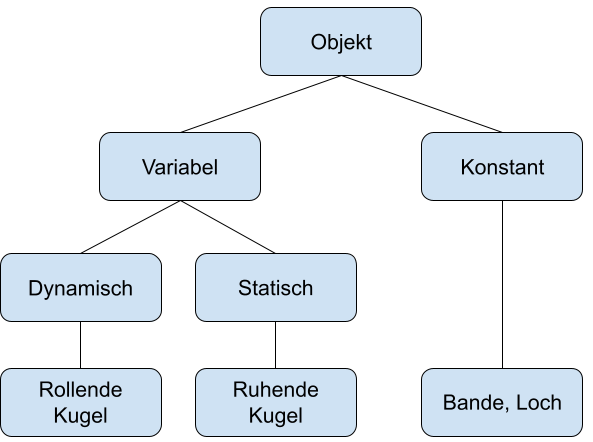
\includegraphics[width=0.5\linewidth]{../common/03_billiard_ai/resources/17_physical_model_categories.png}
    \end{center}
    \caption{Typen von Objekten}
    \label{fig:physical_model_object_categories}
\end{figure}

\newpage
\subsection{Ereignisse und ihre Repräsentation}
Das Ziel ist der Aufbau eines graphenähnlichen Konstrukts, welches aus Layern besteht und Zustandsübergänge variabler
Objekte durch Knoten repräsentiert.
Einige dieser Knoten treten bei Ereignissen wie einer Kollision oder wenn eine Kugel in ein Loch rollt auf.
Andere Knoten dienen der reinen Abbildung des variablen Objekts innerhalb des Layers.
Nachfolgend werden die Knoten definiert.

\begin{minipage}[t]{0.2\textwidth}
    \begin{center}
        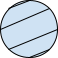
\includegraphics[width=0.3\linewidth]{../common/03_billiard_ai/resources/04_energy_input_node.png}
    \end{center}
\end{minipage}\hfill
\begin{minipage}[t]{0.8\textwidth}
    \textbf{Energy-Input-Node}: Dieser Node beschreibt das Auftreten eines Energie-Inputs von Aussen.
    Beispielsweise wenn die weisse Kugel mit dem Queue gestossen wird.
\end{minipage}\vskip.2\baselineskip
\begin{minipage}[t]{0.2\textwidth}
    \begin{center}
        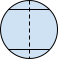
\includegraphics[width=0.3\linewidth]{../common/03_billiard_ai/resources/05_energy_transfer_node.png}
    \end{center}
\end{minipage}\hfill
\begin{minipage}[t]{0.8\textwidth}
    \textbf{Energy-Transfer-Node (Collision-Node)}: Dieser Node beschreibt die Übergabe von Energie auf die
    beteiligten Objekte. Ein Beispiel ist die Kollision zweier Kugeln, wobei diese Energie austauschen.
\end{minipage}\vskip.2\baselineskip
Der Energy-Transfer-Node wird in drei Schichten aufgeteilt. Bei der Input-Schicht wird die Kantenfunktion (siehe S. \pageref{cust:Kantenfunktion})
angewendet. Diese berücksichtigt den Energieverlust bis zum Auftreten des Ereignisses. Die mittlere Schicht beschreibt
die Übergabefunktion der beteiligten Objekte. Die dritte Schicht repräsentiert das Resultat, also den Status der
Objekte nach der Energieübergabe.
\begin{figure}[h!]
    \begin{center}
        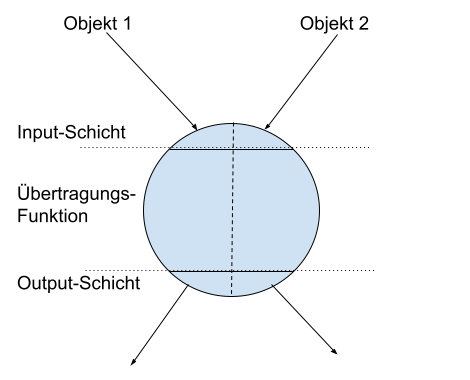
\includegraphics[width=0.5\linewidth]{../common/03_billiard_ai/resources/09_collision_node_description.png}
    \end{center}
    \caption{Der Energy-Transfer-Node}
    \label{fig:Der Energy-Transfer-Node}
\end{figure}\\
\begin{minipage}[t]{0.2\textwidth}
    \begin{center}
        
\includegraphics[width=0.3\linewidth]{../common/03_billiard_ai/resources/06_no_energy_node.png}
    \end{center}
\end{minipage}\hfill
\begin{minipage}[t]{0.8\textwidth}
    \textbf{No-Energy-Node}: Dieser Node wird eingesetzt, sobald der Energiewert eines variablen Objekts auf 0 sinkt und
    somit auch den Übergang von dynamisch zu statisch repräsentiert.
\end{minipage}\vskip.2\baselineskip
\begin{minipage}[t]{0.2\textwidth}
    \begin{center}
        
\includegraphics[width=0.3\linewidth]{../common/03_billiard_ai/resources/07_out_of_system_node.png}
    \end{center}
\end{minipage}\hfill
\begin{minipage}[t]{0.8\textwidth}
    \textbf{Out-Of-System-Node}: Dieser Node wird eingesetzt, sobald ein variables Objekt das System verlässt,
    indem beispielsweise eine Kugel in ein Loch rollt.
\end{minipage}\vskip.2\baselineskip
\begin{minipage}[t]{0.2\textwidth}
    \begin{center}
        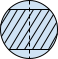
\includegraphics[width=0.3\linewidth]{../common/03_billiard_ai/resources/08_cutting_node.png}
    \end{center}
\end{minipage}\hfill
\begin{minipage}[t]{0.8\textwidth}
    \textbf{Cutting-Node}: Dieser Node ist ein spezieller Energy-Transfer-Node. Er wird bei variablen Objekten
    eingesetzt, die nicht an einem Ereignis beteiligt sind, wenn ein solches auftritt. Zum Ereigniszeitpunkt wird
    ein neuer Layer (siehe S. \pageref{cust:Layer}) geschaffen, welcher die Objekte, die am Ereignis beteiligt sind,
    in einem Energy-Transfer-Node festhält. Weiterhin wird der Status aller dynamsichen Objekte ebenfalls zu diesem
    Zeitpunkt festgehalten. Der Cutting-Node beschränkt sich auf ein Input- sowie Output-Objekt und beinhaltet als
    Energieübertragungsfunktion die Identitätsfunktion.
\end{minipage}\vskip.2\baselineskip

\subsection{Kantenfunktion} \label{cust:Kantenfunktion}
Die Kantenfunktion beschreibt eine Energieabnahme über die Zeit oder den Weg.

\subsection{Layer} \label{cust:Layer}
Ein Layer beinhaltet sämtliche Veränderungen der variablen Objekte und beschreibt den Status aller Objekte zu diesem Zeitpunkt.
Sobald ein Ereignis auftritt wird ein neuer Layer im Modell eingefügt.

\subsection{Beispiel eines Graphen}
Das beschriebene Datenmodell kann als Graph\footnote{Aus effizientsgründen wird auf einen Graphen in der Implementation
verzichtet. Das Modell setzt sich aus verschiedenen Layern zusammen, bei welchen die Informationen der Events für jedes
variable Objekt separat und mit Zugriffszeit $O(1)$ abgelegt werden.} visualisiert werden. Als Beispiel wird die Idee
eines Billardstosses in Abbildung \ref{fig:Beispiel für ein Resultat des Algorithmus phys_sys} hinzugezogen.
Auf dem Tisch liegt eine weisse wie auch zwei rote Kugeln. Die zweite rote Kugel wird an keiner Interaktion beteiligt sein,
weswegen sie ihren Zustand nie verändert. Es ist ersichtlich, dass bei jedem Ereignis für diese Kugel ein \glqq Out-of-energy-Node\grqq{}
eingefügt wird.
Das erste Event beschreibt die Kollision des dynamischen Objekts \glqq weisse Kugel\grqq{} sowie des
statischen Objekts \glqq rote Kugel\grqq{}. Danach verliert die weisse Kugel sämtliche Energie und wechselt in den
Status \glqq Out-of-energy\grqq{}. Da die rote Kugel zu diesem Zeitpunkt dynamisch ist, wird für sie ein
\glqq Cutting-Node\grqq{} eingefügt. Zuletzt rollt die rote Kugel in das Loch, für sie wird ein \glqq Out-of-system-Node\grqq{}
erstellt und das System hat sämtliche Energie verloren. Ein Endzustand wurde erreicht, da alle Kugeln nun statisch sind.

\begin{figure}[h!]
    \begin{center}
        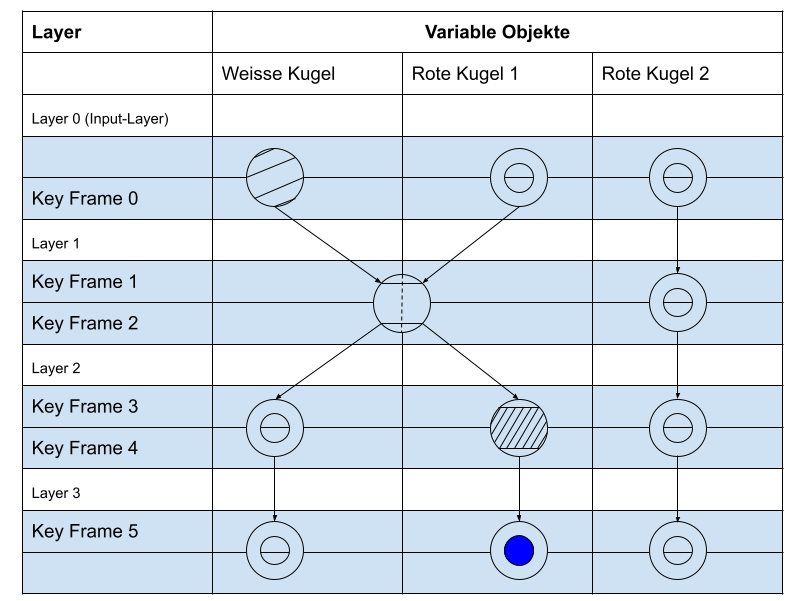
\includegraphics[width=0.6\linewidth]{../common/03_billiard_ai/resources/10_datenmodell_beispiel.png}
    \end{center}
    \caption{Beispiel für ein Resultat des Algorithmus \ref{alg:physikalisches_system}}
    \label{fig:Beispiel für ein Resultat des Algorithmus phys_sys}
\end{figure}

\begin{algorithm}[H]
    \DontPrintSemicolon
    \SetKwFunction{simulate}{simulate}
    \SetKwFunction{nextEvent}{nextEvent}
    \SetKwProg{Fn}{Function}{}{}
    \Fn{\simulate{start: Layer, constantObjects: list} $\longrightarrow$ System}{
        system $\longleftarrow$ System()\\
        system $\longleftarrow$ appendLayer(system, start)\\
        \While{! system.isStatic()}{
            nextEvent $\longleftarrow$ nextEvent(system.lastLayer(), constantObjects)\\
            layer $\longleftarrow$ atMoment(nextEvent)\\
            system $\longleftarrow$ appendLayer(system, start)
        }
        \KwRet system
    }
    \;
    \Fn{\nextEvent{layer: Layer, constantObjects: list} $\longrightarrow$ Node}{
        nextEvent: Node $\longleftarrow$ none\\
        \For{object in layer.dynamicObjects()}{
            nextEvent $\longleftarrow$ min(nextEvent, outOfEnergy(object))\\
            nextEvent $\longleftarrow$ min(nextEvent, collision(object, layer.dynamicObjects()))\\
            nextEvent $\longleftarrow$ min(nextEvent, collision(object, layer.staticObjects()))\\
            nextEvent $\longleftarrow$ min(nextEvent, collision(object, constantObjects))
        }
        \KwRet nextEvent
    }
    \caption{Algorithmus zum Aufbau eines physikalischen Systems}
    \label{alg:physikalisches_system}
\end{algorithm}
In Algorithmus \ref{alg:physikalisches_system} wird die Grundidee erläutert. Als Input für die Funktion \glqq simulate\grqq{}
dient der erste Layer, welcher mehrere variable Objekte beinhalten kann, wobei mindestens ein Objekt dynamisch (energiereich)
sein sollte. Dieser Layer wird direkt dem erzeugten System hinzugefügt und dieses wird solange bearbeitet, bis alle variablen
Objekte statisch sind (das System hat keine Energie mehr). In jedem Schleifendurchlauf wird das nächste Event berechnet.
Die Events können diverser Natur sein. Es werden Kollisionen mit dynamischen, statischen wie auch konstanten Objekten
geprüft. Bei der Kollision mit konstanten Objekten können die Ereignisse \glqq Energy transfer\grqq{} oder \glqq Out of
System\grqq{} auftreten. Weiterhin wird geprüft, ob ein dynamisches Objekt seine Energie durch die Kantenfunktion
verliert.
Aufgrund eines Ereignisses wird zunächst ein neuer Layer generiert, dann für die am Ereignis beteiligten Objekte
den entsprechenden Node und zuletzt für die anderen variablen Objekte entweder ein \glqq Cutting-Node\grqq{} oder ein
\glqq Out-of-energy-Node\grqq{} eingefügt.
